\documentclass[10pt,german,a4paper]{scrreprt}

\usepackage[ngerman]{babel}
\usepackage[utf8]{inputenc} 
\usepackage{lmodern}
\usepackage{listings}
\usepackage{color}
\usepackage{amsmath}
\usepackage{amsthm}
\usepackage{amssymb}
\usepackage{pdfpages}
\usepackage{geometry}
\usepackage{fancyhdr}
\usepackage{graphicx}
\usepackage{hyperref} 
\usepackage{float}		
\usepackage{relsize}		
\usepackage{euscript}	


\hypersetup{
	pdfborder=0
}

\geometry{a4paper,left=1cm,right=1cm, top=2cm, bottom=2cm} 

\def \Path {/media/Daten/Studium/Skripte/Datenbanken}
\makeatletter
	\@addtoreset{chapter}{part}
\makeatother



\title{Architektur von Datenbanksystemen\\Skript}
\subtitle{In der Hoffnung, dass es was nützt ...}
\author{Christian Kroh}
\date{\today{}, Dresden}







\pagestyle{fancy}
\lhead{Skript Architektur von Datenbanksystemen}
\chead{}
\rhead{\leftmark}
\lfoot{Christian Kroh \texttt{(s1428123)}}
\cfoot{}
\rfoot{\thepage}

\renewcommand*{\chapterpagestyle}{fancy}


\newtheoremstyle{mytheoremstyle} % name
    {\topsep}                    % Space above
    {\topsep}                    % Space below
    {\itshape}                   % Body font
    {}                           % Indent amount
    {\scshape}                   % Theorem head font
    {:\\\noindent\makebox[\linewidth]{\rule{\linewidth}{0.4pt}}\\}                          % Punctuation after theorem head
    {.5em}                       % Space after theorem head
    {{\normalfont\bfseries Definition\thmnumber{ #2}\thmnote{ (#3)}: \thmname{#1}}}  % Theorem head spec (can be left empty, meaning ‘normal’)

\theoremstyle{mytheoremstyle}













\begin{document}
\maketitle
\newpage
\tableofcontents
\newpage

\chapter{Allgemeine Einführung}
\section{Qualifikationsziele}
Die Lehrveranstaltung widmet sich im Wesentlichen der Architektur von Datenbanken, wobei die Thematik von unterschiedlichen Perspektiven betrachtet wird.  Zum einen wird der Aufbau traditioneller Datenbanksysteme schrittweise hinsichtlich der verschiedenen funktionalen Schichten diskutiert, wobei datenbankspezifische Konzepte der Externspeicherverwaltung, des Systempuffer-Managements und der internen Satzschnittstelle ausführlich untersucht werden.  Des Weiteren werden orthogonale Konzepte wie aus dem Bereich der parallelen Datenbankarchitektur (Parallelisierung von Datenbankoperatoren) und aus dem Umfeld verteilter Sperr- und Cache-Synchronisationsverfahren betrachtet. Ebenfalls werden im Bereich der verteilten Datenbanken notwendige Technologien für einen zuverlässigen transaktional ausgerichteten Betrieb aufgearbeitet (2-Phasen-Commit-Protokoll, Replikation, etc.). Neben den traditionellen Datenbanksystemen wird auch auf alternative Konzepte, wie z.B. „Column-Store“ Datenbanken und Datenstromsysteme eingegangen. Außerdem werden Prinzipien und Techniken wie Fragmentierung, Replikation, Virtualisierung, Multi-Tenancy oder CAP-Theorem sowohl im Bezug auf operationale wie auch auf analytische Probleme diskutiert.\\\\
Datenbank- und Informationssysteme können in zwei große Bestandteile zerlegt werden. Auf der einen Seite steht das Speichermanagement, d.h. die Komponenten, die für die physische Organisation der Datenbestände zur Verfügung stehen. Die unterschiedlichen Methoden und Komponenten werden dabei im ersten Teil der Vorlesungsreihe besprochen. Auf der anderen Seite steht die Verarbeitungseinheit, also die Komponenten eines Systems, die transaktional geschützt, nebenläufig korrekt und effizient Datenbankanfragen bearbeiten. Die Methoden und die Aufgaben der unterschiedlichen Komponenten werden in diesem zweiten Teil der Vorlesung besprochen. Als Schnittstelle zwischen den Schichten innerhalb der Datenbankarchitektur dient die Auffassung eines Key-Value-Paares. Dabei kann Key-Value bedeuten, dass dies direkt von der Applikation genutzt bzw. programmiert werden kann oder höhere Systemschichten darauf aufsetzen. Ziel der Vorlesung ist es ein tiefes Verständnis von Anfrageverarbeitungs- und optimierungstechniken unter den Randbedingungen transaktionaler Korrektheit zu vermitteln.

\section{Basisliteratur}
\begin{itemize}
\item A. Kemper, A. Eickler: “Datenbanksysteme”, Oldenbourg-Verlag
\item R. Elmasri and S. Navathe: “Grundlagen von Datenbanksystemen”, 3. überarbeitete
Auflage, Addison-Wesley, 2002
\end{itemize}

\section{Spezielle Literatur}
\begin{itemize}
\item Gunter Saake, Andreas Heuer, Kai-Uwe Sattler: Datenbanken:
Implentierungstechniken, mitp Verlag, 2. Auflage

\item Härder T.; Rahm, E.: Datenbanksysteme. Konzepte und Techniken der
Implementierung, Springer-Verlag
\item Ramakrishnan, R.; Gehrke, J.: “Database Management Systems”. McGraw-Hill, 2000

\end{itemize}

\newpage
\part{Allgemeines}
\newpage
\chapter{Datenbanksystem}

	\newtheorem{db-def}{Datenbanksystem}
	\begin{db-def}
		ein System zur Beschreibung, Speicherung und Wiedergewinnung von umfangreichen Datenmengen, die von mehreren Anwendungsprogrammen genutzt werden
	\end{db-def}
	
	\paragraph{Komponenten}
	\begin{itemize}
		\item Datenbank, in der die Daten abgelegt werden
		\item Datenbanksoftware, die die Daten entsprechend den vorgegebenen Beschreibungen abspeichern, auffinden oder weitere Operationen mit den Daten durchführen
	\end{itemize}
	
	\paragraph{Leistung in den folgenden Bereichen}
	\begin{itemize}
		\item Datenmodell und Datendefinition
		\item Datenzugriff und -manipulation
		\item Steuerung und Überwachung
	\end{itemize}

\chapter{Datenbankanfragen}
	
\section{Anfragesprachen}
	\subsection{Typen von Anfragesprachen}
	\begin{itemize}
		\item Prozedurale Datenbanksprachen
		\begin{itemize}
			\item Tupel- oder Satzorientiert
			\item Programmierer denkt in Satzfolgen
			\item Navigation über Zugriffspfade durch die vorhandenen Daten\\findNext()\\findFirst()
		\end{itemize}
		\item Deskreptive Datenbanksprachen
		\begin{itemize}
			\item Mengenorientiert (typisch für Relationenmodell)
			\item Programmierer denkt in Mengen von Sätzen mit bestimmten Eigenschaften
			\item Zugriff erfolgt durch inhaltliche Kriterien
		\end{itemize}
	\end{itemize}
	
	\subsubsection{Beispiel SQL}
		\paragraph{DDL (Data Definition Language)}
		\paragraph{DML (Data Manipulation Language)}
	
	\subsection{Optimierungsarten}

\section{Anfrageverarbeitung}

\chapter{Komponenten eines Datenbanksystems}
	\begin{center}
		\includegraphics[page=23, width=0.49\linewidth, trim=5mm 15mm 5mm 25mm, clip]{\Path/Vorlesung/ADBS-1/01_Einfuehrung.pdf}
		\includegraphics[page=24, width=0.49\linewidth, trim=5mm 15mm 5mm 25mm, clip]{\Path/Vorlesung/ADBS-1/01_Einfuehrung.pdf}
	\end{center}

\chapter{Schichtenmodell}



\part{ADBS-1: Betriebssystem, Puffer- und Speicherverwaltung}
\newpage
\chapter{Einführung}
\section{Themenschwerpunkte}
	\begin{description}

		\item[Verarbeitungsleistung]\hfill
			\\\textbf{Im Vordergrund stehen:}
			\begin{itemize}
				\item Schnelle Verarbeitung auch einzelner Bits
				\item Parallelität auf: \hfill
				\begin{itemize}
					\item Bitebene
					\item Befehlseben
					\item Threadebene
					\item Prozess- und Anwendungsebene
				\end{itemize}
				\item dynamische Rekonfiguration
			\end{itemize}
			$\Rightarrow$ Erfüllung der gegebenen Anforderungen

		\item[Systemintegration]\hfill
			\\\textbf{Im Vordergrund stehen:}
			\begin{itemize}
				\item Mehrprozessorsyteme, Mehrkern-, Vielkernprozessorsysteme
				\item Mehr-Chip- / Einzel-Chip-Lösungen (System-on-a-Chip)
				\item Parallele Entwicklung von HW und SW
	(HW-/SW-Codesign)
				\item System-Prototyping (FPGA-Entwurf)
			\end{itemize}
			$\Rightarrow$ Kosteneinsparung, Entwicklungszeiteinsparung (Time-to-Market)

		\item[Verlustleistung]
			\hfill\\\textbf{Im Vordergrund stehen:}
			\begin{itemize}
				\item Verlustleistung im Standby (Akkubetrieb)
				\item Maximales Abwärmebudget
			\end{itemize}

			\hfill\\\textbf{Kenngrößen:}
			\begin{itemize}
				\item Statische und dynamische Verlustleistung
				\item MIPS pro Watt
			\end{itemize}

			$\Rightarrow$ Sowohl für eingebettete Systeme als auch für Server


		\item[Korrektheit]
			\hfill\\\textbf{Aspekte:}
			\begin{itemize}
				\item Verifikation eines Schaltkreises, simulativ / formal
				\item Profiling und Debugging unter Echtzeitbedingungen (Trace)
			\end{itemize}
			$\Rightarrow$ Fehlerfreier Erstentwurf


		\item[Fehlertoleranz]\hfill
			\\\textbf{Toleranz gegenüber:}
			\begin{itemize}
				\item Permanenten Fehlern (zeitunabhängig nach erstem Auftreten)
				\item Intermitierenden Fehlern (nur unter bestimmten Betriebsbedingungen)
				\item Transienten Fehlern (aufgrund statischer Störungen)
			\end{itemize}

			\hfill\\\textbf{Fehlererkennung und -korrektur:}
			\begin{itemize}
				\item Autonom durch Hardwarearchitektur
				\item Aus Kombination von HW und SW
			\end{itemize}

			$\Rightarrow$ Insbesondere wichtig für Sicherheitskritische, hochverfügbare und langlebige zuverlässige Systeme
			\\$\Rightarrow$ Steigende Siginifikanz mit abnehmenden Strukturgrößen (Integrationsgrad) sowie steigender Transistoranzahl (Moore's Law)
	\end{description}


\section{Inhalte der Lehrveranstaltung}
\subsection{Inhalte der Vorlesung}
	\begin{enumerate}
		\item Klassifikation von Schaltkreisen
		\item Grundlagen des Schaltkreisentwurfs
		\item Automatendarstellung, -kopplung, -vereinfachung
		\item Hardwarebeschreibungssprachen
		\item Programmierabare Schaltkreise, insbesondere FPGAs - Teil 1
		\item Programmierabare Schaltkreise, insbesondere FPGAs - Teil 2
		\item Modellierung und Simulation
		\item Zeitverhalten und Test
		\item Hochgeschwindigkeit und Verlsustleistung
		\item Anwendungsbeispiele
	\end{enumerate}

\subsection{Inhalte des Praktikums}
	\begin{enumerate}
		\item Altera Quartus-Toolchain \& Praktikumsboard DE0 mit Cyclone-3
		\item Schaltnetze und Schaltwerke
		\item Modularisierung
		\item \grqq Komplexe\grqq Anwendung: Stoppuhr
	\end{enumerate}


\section{Klassifikation von ICs}

\subsection{Zwei Sichten}
	\hfill\\Klassifizierung von integrierten Schaltkreisen (ICs) in
	\begin{itemize}
		\item Standarschaltkreis (Standard-IC) und
		\item applikationspezifische Schaltkreise (Application-Specific IC, \textbf{ASIC})
	\end{itemize}
	unter zwei Gesichtspunkten möglich:
	\begin{itemize}
		\item \textbf{Herstellungssicht}
		\item \textbf{Entwurfssicht}
	\end{itemize}

	\paragraph{Herstellungssicht:}
	\begin{itemize}
		\item Standard-IC = große Stückzahl für viele Kunden
		\item ASIC = für eine/n Kunden/Applikation speziell entwickelter und gefertigter IC mit zugeschnittener Funktionalität
	\end{itemize}

	\paragraph{Entwurfssicht:}
	\begin{itemize}
		\item Standard-IC = (Hardware-)Funktionalität kann nicht vom Anwender beeinflusst werden
		\item ASIC = vom Anwender selbst entwickelte (Hardware-)Funktionalität
	\end{itemize}

	\newpage
	\begin{center}
	\includegraphics[page=17, width=0.7\linewidth, trim=30mm 20mm 20mm 40mm, clip]{\Path/resources/Vorlesung/VLSI/01_Einfuehrung.pdf}
	\\\includegraphics[page=18, width=0.7\linewidth, trim=30mm 20mm 20mm 40mm, clip]{\Path/resources/Vorlesung/VLSI/01_Einfuehrung.pdf}
	\\\includegraphics[page=19, width=0.7\linewidth, trim=30mm 20mm 20mm 40mm, clip]{\Path/resources/Vorlesung/VLSI/01_Einfuehrung.pdf}
	\end{center}

\subsection{Anwenderprogrammierbare IC (ASIC)}
	\paragraph{Merkmale:}
	\begin{itemize}
		\item Field-Programmable $\Leftrightarrow$ feldprogrammierbar
		\item Vor Ort (im Feld) vom Anwender programmierbar
		\item Hardware ist fix. Funktionalität kann aber mittels spezieller Konfiguration \grqq programmiert\grqq werden
	\end{itemize}
	\paragraph{Anwendung:}
	\begin{itemize}
		\item Anwendungsspezifische IC bei kleinen und mittleren Stückzahlen
		\item Mehrfach neu programmierbar zwecks Optimierung und Fehlerbehebung, auch während des praktischen Einsatzes
		\item Einfache Integration eines ganzen Systems auf einem Chip
		\item Prototyping, HW-/SW-Codesign
	\end{itemize}

\subsection{Hardwareprogrammierung}
	\begin{center}
	\includegraphics[page=21, width=0.7\linewidth, trim=30mm 20mm 20mm 40mm, clip]{\Path/resources/Vorlesung/VLSI/01_Einfuehrung.pdf}
	\end{center}
%\newpage
\subsection{Programmiertechnologien}
	\begin{center}
	\includegraphics[page=22, width=0.7\linewidth, trim=30mm 20mm 20mm 40mm, clip]{\Path/resources/Vorlesung/VLSI/01_Einfuehrung.pdf}
	\\\includegraphics[page=23, width=0.7\linewidth, trim=30mm 20mm 20mm 40mm, clip]{\Path/resources/Vorlesung/VLSI/01_Einfuehrung.pdf}
	\\\includegraphics[page=24, width=0.7\linewidth, trim=30mm 20mm 20mm 40mm, clip]{\Path/resources/Vorlesung/VLSI/01_Einfuehrung.pdf}
	\\\includegraphics[page=25, width=0.7\linewidth, trim=30mm 20mm 20mm 40mm, clip]{\Path/resources/Vorlesung/VLSI/01_Einfuehrung.pdf}
	\\\includegraphics[page=26, width=0.7\linewidth, trim=30mm 20mm 20mm 40mm, clip]{\Path/resources/Vorlesung/VLSI/01_Einfuehrung.pdf}
	\\\includegraphics[page=27, width=0.7\linewidth, trim=30mm 20mm 20mm 40mm, clip]{\Path/resources/Vorlesung/VLSI/01_Einfuehrung.pdf}
	\\\includegraphics[page=28, width=0.7\linewidth, trim=30mm 20mm 20mm 40mm, clip]{\Path/resources/Vorlesung/VLSI/01_Einfuehrung.pdf}
	\end{center}

\subsection{Klassifikation Anwenderprogrammierbare IC}
	\begin{center}
	\includegraphics[page=29, width=0.7\linewidth, trim=30mm 20mm 20mm 40mm, clip]{\Path/resources/Vorlesung/VLSI/01_Einfuehrung.pdf}
	\\\includegraphics[page=30, width=0.7\linewidth, trim=30mm 20mm 20mm 40mm, clip]{\Path/resources/Vorlesung/VLSI/01_Einfuehrung.pdf}
	\\\includegraphics[page=31, width=0.7\linewidth, trim=30mm 20mm 20mm 40mm, clip]{\Path/resources/Vorlesung/VLSI/01_Einfuehrung.pdf}
	\end{center}

\newpage

\chapter{Segment- und Seitenverwaltung}

\chapter{Einbringstrategien}

\chapter{Systempuffer}

\chapter{Row-based Record Management (klassische Satzverwaltung)}

\chapter{Column-based Record Management}

\chapter{Distributed Key-Value Stores}

\chapter{Replication}




\part{ADBS-2: Zugriffssystem, Datensystem}
\newpage
%\input{../Parallelrechner/Skript/00-Parallelrechner}


\part{Appendix}
\newpage
%\input{../Parallelrechner/Skript/00-Parallelrechner}
\end{document}
